\section{Model predictions errors for counties in the United States}

% ERRORS

\begin{landscape}
\begin{table}[!htb]
    \centering
    \begin{tabular}{| c | c | c | c | c | c | c | c | c | c | c |}
        \multirow{2}{*}{Days}
            & \multirow{2}{*}{Loc.}
            & \multicolumn{3}{c |}{Baseline}
            & \multicolumn{3}{c |}{2nd. Ver}
            & \multicolumn{3}{c |}{3rd. Ver} \\ \cline{3-11}
            & & MAE & MAPE & RMSE & MAE & MAPE & RMSE & MAE & MAPE & RMSE \\
        \hline\hline

        \multirow{4}{*}{7}
            & Cook & 5.847 & 0.055 & 6.291 & 18.390 & 0.173 & 19.257 & 21.309 & 0.200 & 22.031
            \\ \cline{2-11}
            & Harris & 46.021 & 0.666 & 50.000 & 38.705 & 0.560 & 43.120 & 32.571 & 0.471 & 36.267
            \\ \cline{2-11}
            & Los Angeles & 28.781 & 0.115 & 31.633 & 51.605 & 0.206 & 54.813 & 50.488 & 0.202 & 53.633
            \\ \cline{2-11}
            & Maricopa & 39.739 & 0.374 & 40.227 & 38.180 & 0.360 & 38.746 & 36.632 & 0.345 & 37.215
            \\
        \hline

        \multirow{4}{*}{14}
            & Cook & 13.181 & 0.123 & 15.800 & 31.772 & 0.297 & 35.375 & 34.551 & 0.323 & 37.832
            \\ \cline{2-11}
            & Harris & 95.339 & 1.355 & 111.180 & 87.944 & 1.249 & 104.920 & 74.010 & 1.052 & 88.397
            \\ \cline{2-11}
            & Los Angeles & 54.539 & 0.217 & 61.814 & 87.975 & 0.350 & 97.176 & 86.045 & 0.343 & 95.029
            \\ \cline{2-11}
            & Maricopa & 55.439 & 0.519 & 58.393 & 54.897 & 0.514 & 58.269 & 53.215 & 0.498 & 56.632
            \\
        \hline

        \multirow{4}{*}{21}
            & Cook & 21.380 & 0.199 & 25.491 & 45.720 & 0.426 & 51.581 & 48.620 & 0.453 & 54.215
            \\ \cline{2-11}
            & Harris & 158.343 & 2.205 & 189.162 & 152.570 & 2.123 & 185.661 & 127.313 & 1.772 & 154.368
            \\ \cline{2-11}
            & Los Angeles & 82.513 & 0.327 & 95.410 & 126.976 & 0.503 & 143.413 & 123.921 & 0.491 & 139.857
            \\ \cline{2-11}
            & Maricopa & 76.472 & 0.711 & 83.882 & 77.590 & 0.721 & 86.019 & 75.672 & 0.703 & 84.128
            \\
        \hline

        \multirow{4}{*}{28}
            & Cook & 29.629 & 0.275 & 35.088 & 59.121 & 0.549 & 66.872 & 62.355 & 0.579 & 69.979
            \\ \cline{2-11}
            & Harris & 227.124 & 3.099 & 272.682 & 225.190 & 3.070 & 274.928 & 184.261 & 2.513 & 223.06
            \\ \cline{2-11}
            & Los Angeles & 117.110 & 0.461 & 138.626 & 171.721 & 0.677 & 197.699 & 167.210 & 0.659 & 192.284
            \\ \cline{2-11}
            & Maricopa & 101.192 & 0.933 & 114.101 & 104.663 & 0.965 & 119.407 & 102.385 & 0.944 & 117.066
            \\
        \hline
    \end{tabular}
    \caption{Out-of-sample errors of the model's predictions on the number of deaths for the counties in the United States. The lowest errors for each evaluation metrics at each location are highlighted.}
\end{table}
\end{landscape}

\begin{landscape}
\begin{table}[!htb]
    \centering
    \begin{tabular}{| c | c | c | c | c | c | c | c | c | c | c |}
        \multirow{2}{*}{Days}
            & \multirow{2}{*}{Loc.}
            & \multicolumn{3}{c |}{Baseline}
            & \multicolumn{3}{c |}{2nd. Ver}
            & \multicolumn{3}{c |}{3rd. Ver} \\ \cline{3-11}
            & & MAE & MAPE & RMSE & MAE & MAPE & RMSE & MAE & MAPE & RMSE \\
        \hline\hline

        \multirow{4}{*}{7}
            & Cook & 22.545 & 2.377 & 28.432 & 55.668 & 6.041 & 66.778 & 41.352 & 4.467 & 55.4
            \\ \cline{2-11}
            & Harris & 1022.438 & 30.850 & 1193.354 & 1093.142 & 32.772 & 1280.746 & 1535.176 & 0.333 & 1736.348
            \\ \cline{2-11}
            & Los Angeles & 981.461 & 20.945 & 1140.886 & 1126.805 & 24.141 & 1297.286 & 1082.929 & 23.181 & 1248.996
            \\ \cline{2-11}
            & Maricopa & 95.129 & 4.730 & 99.906 & 19.956 & 0.987 & 23.867 & 19.382 & 0.968 & 21.617
            \\
        \hline

        \multirow{4}{*}{14}
            & Cook & 35.341 & 3.517 & 45.173 & 90.017 & 9.156 & 101.192 & 59.667 & 6.104 & 68.594
            \\ \cline{2-11}
            & Harris & 890.257 & 28.652 & 1093.096 & 984.436 & 30.810 & 1205.333 & 2209.289 & 0.465 & 2506.827
            \\ \cline{2-11}
            & Los Angeles & 698.901 & 15.302 & 950.789 & 802.626 & 17.610 & 1085.485 & 768.943 & 16.918 & 1038.125
            \\ \cline{2-11}
            & Maricopa & 136.130 & 6.883 & 172.143 & 69.022 & 3.427 & 94.846 & 62.939 & 3.176 & 95.737
            \\
        \hline

        \multirow{4}{*}{21}
            & Cook & 70.168 & 7.131 & 92.661 & 136.784 & 14.489 & 177.086 & 96.828 & 10.550 & 144.579
            \\ \cline{2-11}
            & Harris & 715.160 & 23.718 & 932.114 & 963.073 & 32.888 & 1132.567 & 1664.322 & 0.348 & 2097.628
            \\ \cline{2-11}
            & Los Angeles & 477.179 & 10.682 & 776.682 & 557.786 & 12.785 & 887.881 & 584.712 & 14.463 & 857.916
            \\ \cline{2-11}
            & Maricopa & 139.674 & 6.888 & 169.314 & 92.801 & 4.357 & 134.620 & 76.112 & 3.609 & 116.774
            \\
        \hline

        \multirow{4}{*}{28}
            & Cook & 83.696 & 8.105 & 119.396 & 184.792 & 19.135 & 230.863 & 139.144 & 14.665 & 190.726
            \\ \cline{2-11}
            & Harris & 605.536 & 20.796 & 824.160 & 982.211 & 35.537 & 1123.076 & 2479.698 & 0.499 & 3145.165
            \\ \cline{2-11}
            & Los Angeles & 412.908 & 11.617 & 686.484 & 498.917 & 14.897 & 794.110 & 546.785 & 17.824 & 784.312
            \\ \cline{2-11}
            & Maricopa & 217.947 & 11.510 & 271.885 & 129.381 & 104.125 & 5.223 & 109.935 & 5.689 & 149.951
            \\
        \hline
    \end{tabular}
    \caption{Out-of-sample errors of the model's predictions on the number of new cases for the counties in the United States. The lowest errors for each evaluation metrics at each location are highlighted.}
\end{table}
\end{landscape}

\begin{landscape}
\begin{table}[!htb]
    \centering
    \begin{tabular}{| c | c | c | c | c | c | c | c | c | c | c |}
        \multirow{2}{*}{Days}
            & \multirow{2}{*}{Loc.}
            & \multicolumn{3}{c |}{Baseline}
            & \multicolumn{3}{c |}{2nd. Ver}
            & \multicolumn{3}{c |}{3rd. Ver} \\ \cline{3-11}
            & & MAE & MAPE & RMSE & MAE & MAPE & RMSE & MAE & MAPE & RMSE \\
        \hline\hline

        \multirow{4}{*}{7}
            & Cook & 678.757 & 0.117 & 679.641 & 750.786 & 0.130 & 761.605 & 595.890 & 0.103 & 604.919
            \\ \cline{2-11}
            & Harris & 2429.798 & 0.520 & 3193.800 & 2629.532 & 0.562 & 3482.363 & 1535.176 & 0.333 & 1736.348
            \\ \cline{2-11}
            & Los Angeles & 2351.443 & 0.172 & 2920.659 & 2898.771 & 0.212 & 3633.093 & 2545.519 & 0.186 & 3107.429
            \\ \cline{2-11}
            & Maricopa & 1491.513 & 0.242 & 1510.229 & 974.924 & 0.159 & 975.073 & 410.099 & 0.067 & 412.091
            \\
        \hline

        \multirow{4}{*}{14}
            & Cook & 612.953 & 0.105 & 621.265 & 1129.956 & 0.194 & 1212.272 & 874.273 & 0.150 & 928.652
            \\ \cline{2-11}
            & Harris & 5883.932 & 1.224 & 6993.098 & 6824.524 & 1.419 & 8209.270 & 2209.289 & 0.465 & 2506.827
            \\ \cline{2-11}
            & Los Angeles & 5141.081 & 0.371 & 5985.620 & 6376.008 & 0.460 & 7440.514 & 5501.848 & 0.397 & 6381.884
            \\ \cline{2-11}
            & Maricopa & 2026.365 & 0.325 & 2112.334 & 963.663 & 0.155 & 969.336 & 480.406 & 0.077 & 492.111
            \\
        \hline

        \multirow{4}{*}{21}
            & Cook & 465.474 & 0.080 & 519.420 & 1659.534 & 0.282 & 1879.133 & 1219.233 & 0.207 & 1359.485
            \\ \cline{2-11}
            & Harris & 7611.514 & 1.553 & 8583.826 & 9913.906 & 2.017 & 11519.766 & 1664.322 & 0.348 & 2097.628
            \\ \cline{2-11}
            & Los Angeles & 6242.229 & 0.447 & 6903.758 & 7690.419 & 0.551 & 8509.198 & 6313.624 & 0.452 & 6943.113
            \\ \cline{2-11}
            & Maricopa & 2549.187 & 0.402 & 2705.335 & 767.923 & 0.123 & 826.909 & 396.265 & 0.063 & 425.505
            \\
        \hline

        \multirow{4}{*}{28}
            & Cook & 486.964 & 0.083 & 548.673 & 2493.195 & 0.420 & 3000.083 & 1869.379 & 0.315 & 2260.015
            \\ \cline{2-11}
            & Harris & 8785.001 & 1.760 & 9652.091 & 13119.518 & 2.612 & 15167.205 & 2479.698 & 0.499 & 3145.165
            \\ \cline{2-11}
            & Los Angeles & 6715.207 & 0.478 & 7232.734 & 7974.478 & 0.568 & 8596.755 & 6094.396 & 0.435 & 6615.172
            \\ \cline{2-11}
            & Maricopa & 3327.537 & 0.517 & 3705.984 & 670.792 & 0.107 & 754.504 & 452.858 & 0.071 & 533.121
            \\
        \hline
    \end{tabular}
    \caption{Out-of-sample errors of the model's predictions on the number of cumulative cases for the counties in the United States. The lowest errors for each evaluation metrics at each location are highlighted.}
\end{table}
\end{landscape}

\subsection{Reproduction number and fatality rate}

\begin{figure}[!htb]
    \centering

    \begin{subfigure}[b]{\linewidth}
        \centering
        \begin{subfigure}[b]{0.4\linewidth}
            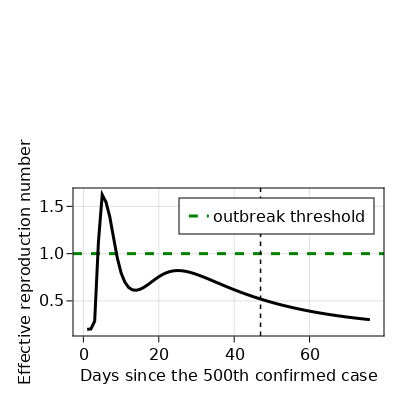
\includegraphics[width=\linewidth]{baseline/cook_il/20211215163025.baseline.cook_il.R_effective.png}
        \end{subfigure}
        \begin{subfigure}[b]{0.4\linewidth}
            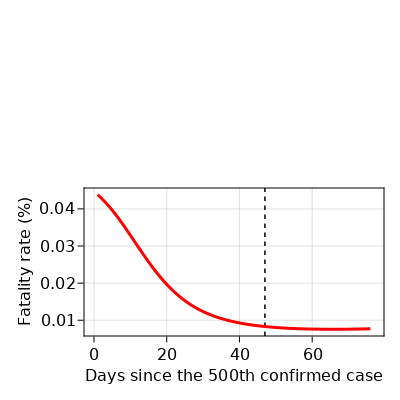
\includegraphics[width=\linewidth]{baseline/cook_il/20211215163025.baseline.cook_il.fatality_rate.png}
        \end{subfigure}
        \subcaption{Baseline model}
    \end{subfigure}

    \begin{subfigure}[b]{\linewidth}
        \centering
        \begin{subfigure}[b]{0.4\linewidth}
            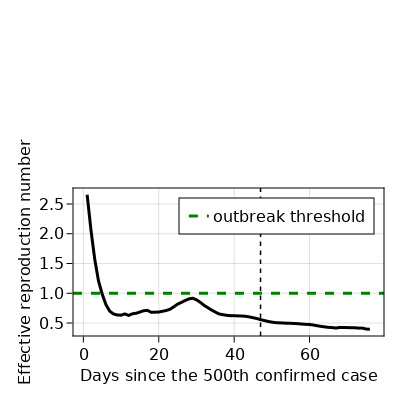
\includegraphics[width=\linewidth]{fb1/cook_il/20211216131821.fbmobility1.cook_il.R_effective.png}
        \end{subfigure}
        \begin{subfigure}[b]{0.4\linewidth}
            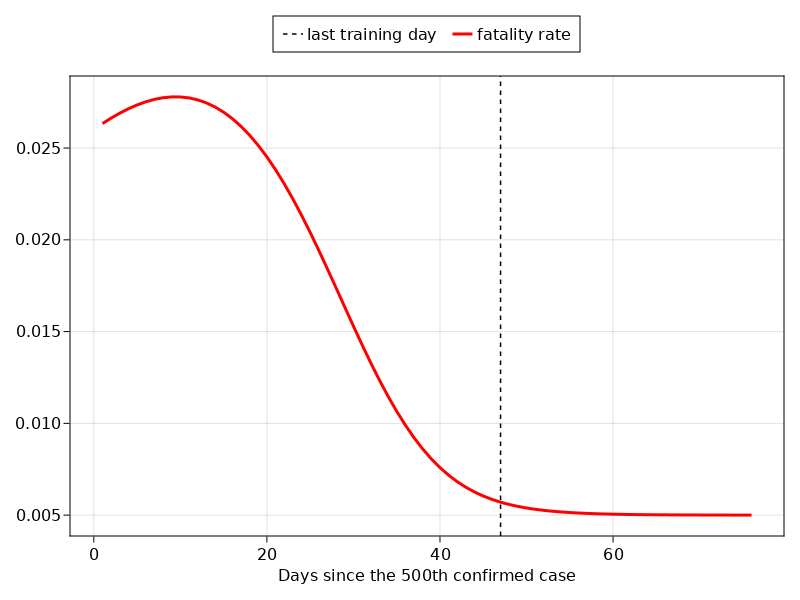
\includegraphics[width=\linewidth]{fb1/cook_il/20211216131821.fbmobility1.cook_il.fatality_rate.png}
        \end{subfigure}
        \subcaption{2nd. version}
    \end{subfigure}

    \begin{subfigure}[b]{\linewidth}
        \centering
        \begin{subfigure}[b]{0.4\linewidth}
            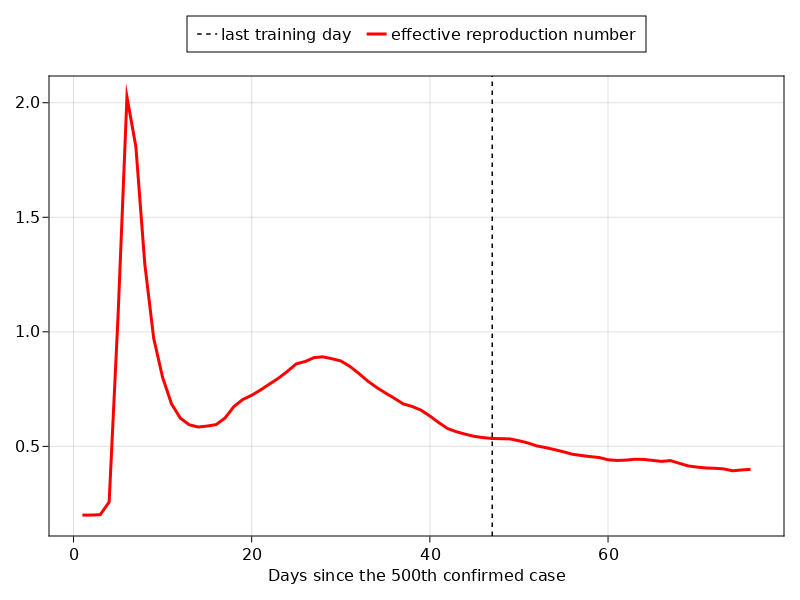
\includegraphics[width=\linewidth]{fb2/cook_il/20211216142727.fbmobility2.cook_il.R_effective.png}
        \end{subfigure}
        \begin{subfigure}[b]{0.4\linewidth}
            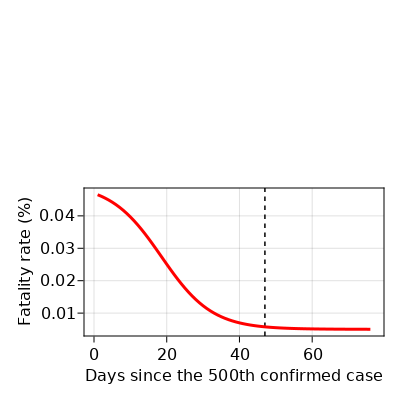
\includegraphics[width=\linewidth]{fb2/cook_il/20211216142727.fbmobility2.cook_il.fatality_rate.png}
        \end{subfigure}
        \subcaption{3rd. version}
    \end{subfigure}

    \caption{The effective reproduction number and the fatality rate for Cook (Illinois), learned by different versions of the model}
    \label{fig:R0-and-fatality-cook}
\end{figure}

\begin{figure}[!htb]
    \centering

    \begin{subfigure}[b]{\linewidth}
        \centering
        \begin{subfigure}[b]{0.4\linewidth}
            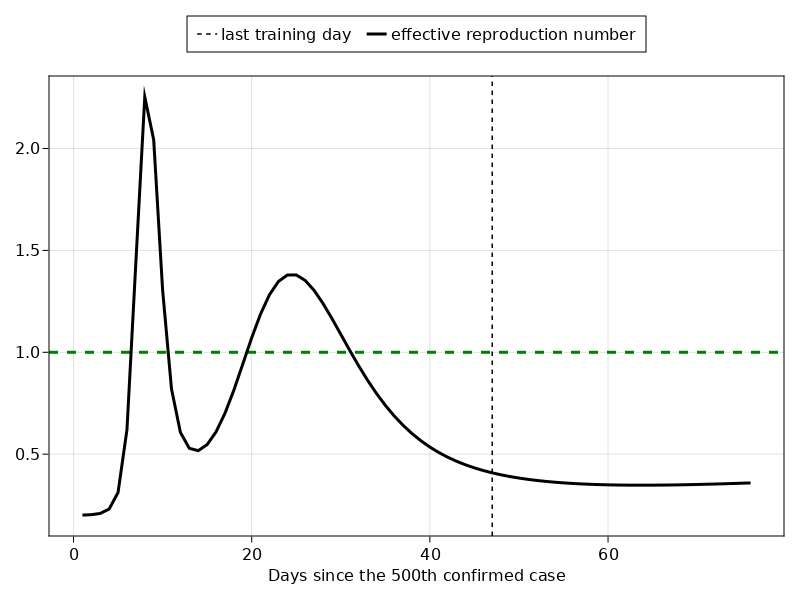
\includegraphics[width=\linewidth]{baseline/harris_tx/20211216154445.baseline.harris_tx.R_effective.png}
        \end{subfigure}
        \begin{subfigure}[b]{0.4\linewidth}
            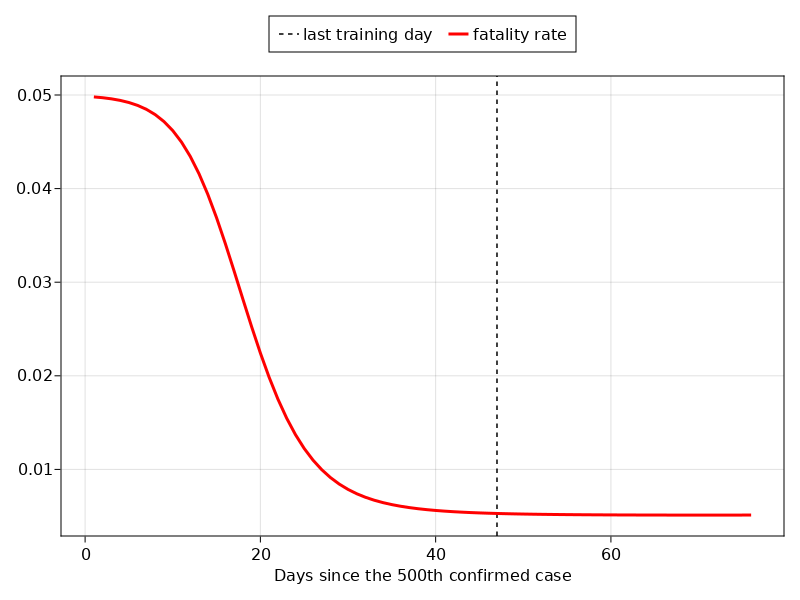
\includegraphics[width=\linewidth]{baseline/harris_tx/20211216154445.baseline.harris_tx.fatality_rate.png}
        \end{subfigure}
        \subcaption{Baseline model}
    \end{subfigure}

    \begin{subfigure}[b]{\linewidth}
        \centering
        \begin{subfigure}[b]{0.4\linewidth}
            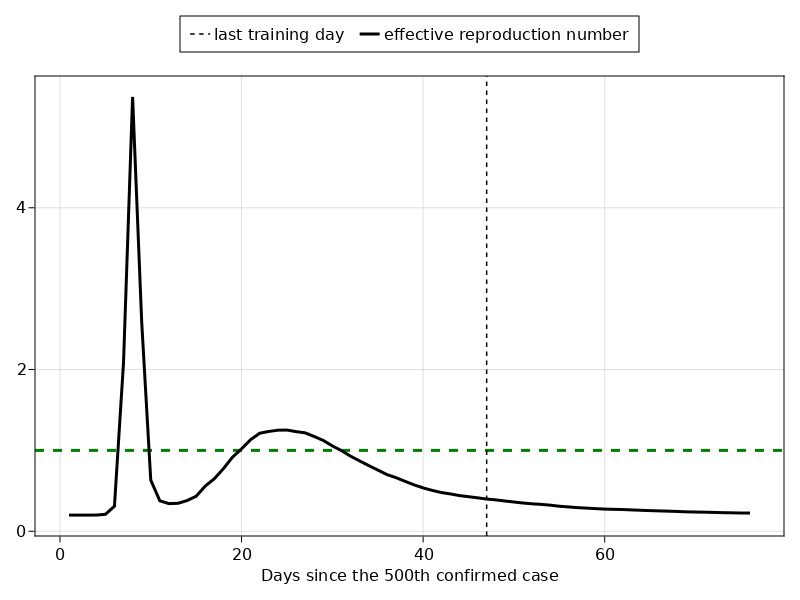
\includegraphics[width=\linewidth]{fb1/harris_tx/20211216231719.fbmobility1.harris_tx.R_effective.png}
        \end{subfigure}
        \begin{subfigure}[b]{0.4\linewidth}
            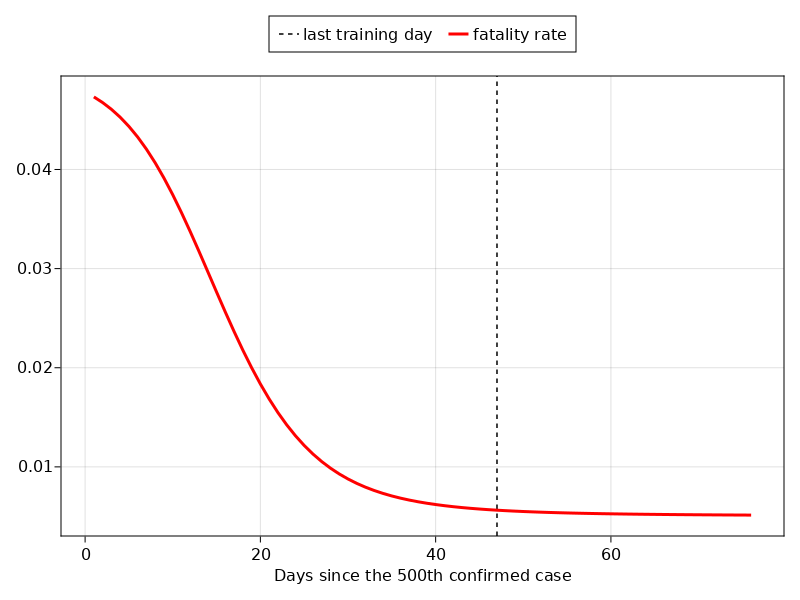
\includegraphics[width=\linewidth]{fb1/harris_tx/20211216231719.fbmobility1.harris_tx.fatality_rate.png}
        \end{subfigure}
        \subcaption{2nd. version}
    \end{subfigure}

    \begin{subfigure}[b]{\linewidth}
        \centering
        \begin{subfigure}[b]{0.4\linewidth}
            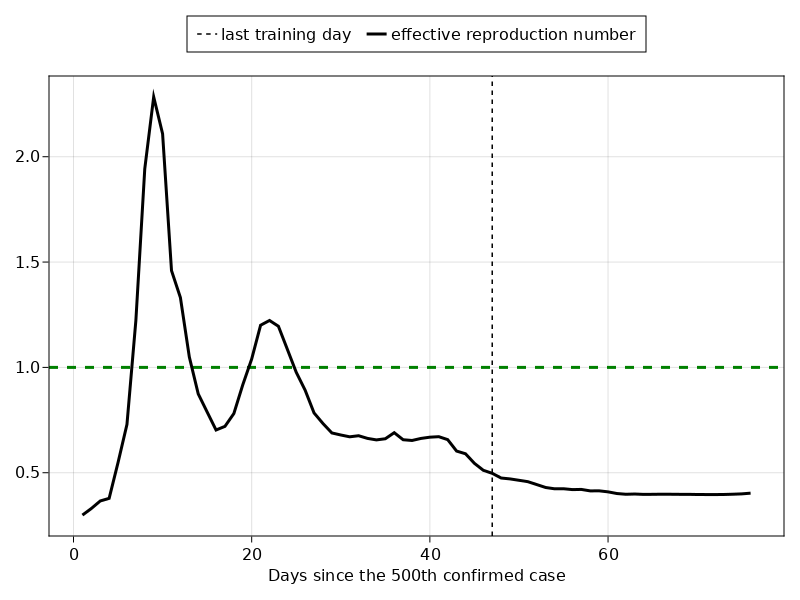
\includegraphics[width=\linewidth]{fb2/harris_tx/20211217204936.fbmobility2.harris_tx.R_effective.png}
        \end{subfigure}
        \begin{subfigure}[b]{0.4\linewidth}
            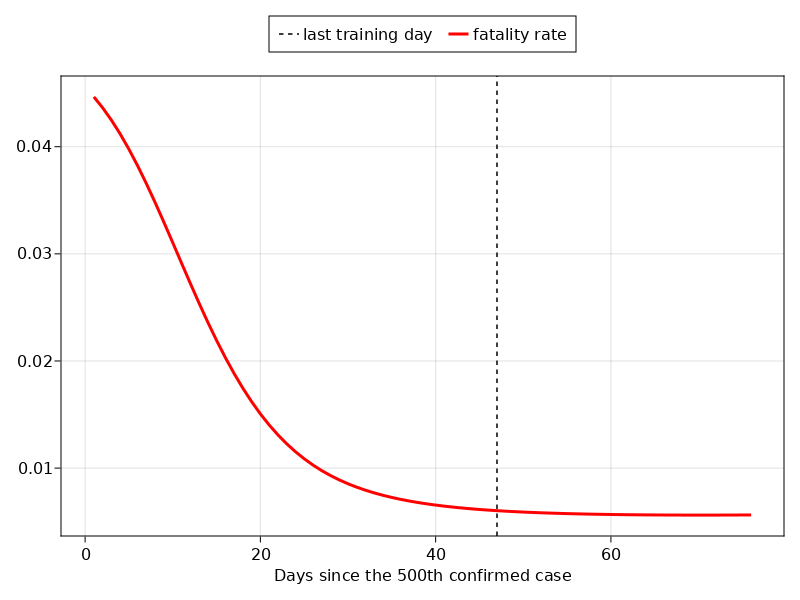
\includegraphics[width=\linewidth]{fb2/harris_tx/20211217204936.fbmobility2.harris_tx.fatality_rate.png}
        \end{subfigure}
        \subcaption{3rd. version}
    \end{subfigure}

    \caption{The effective reproduction number and the fatality rate for Harris (Texas) learned by different versions of the model}
    \label{fig:R0-and-fatality-harris}
\end{figure}


\begin{figure}[!htb]
    \centering

    \begin{subfigure}[b]{\linewidth}
        \centering
        \begin{subfigure}[b]{0.4\linewidth}
            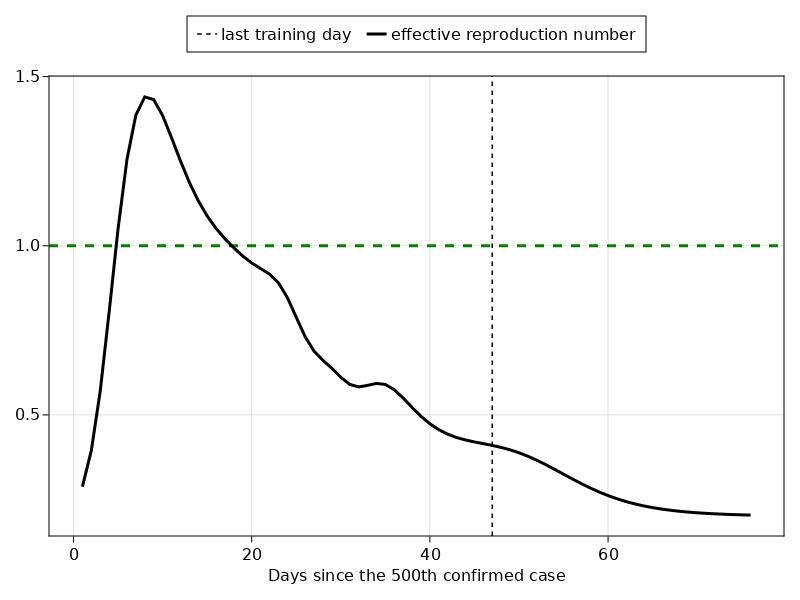
\includegraphics[width=\linewidth]{baseline/losangeles_ca/20211216124108.baseline.losangeles_ca.R_effective.png}
        \end{subfigure}
        \begin{subfigure}[b]{0.4\linewidth}
            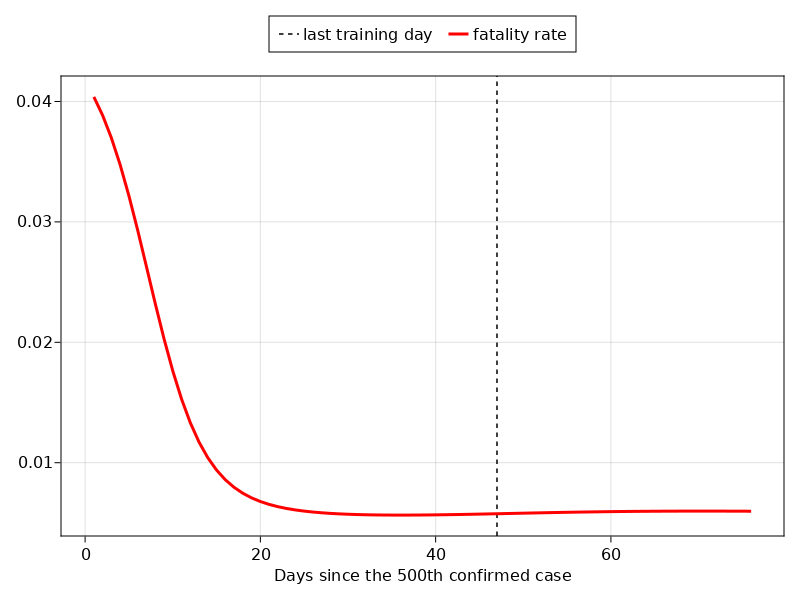
\includegraphics[width=\linewidth]{baseline/losangeles_ca/20211216124108.baseline.losangeles_ca.fatality_rate.png}
        \end{subfigure}
        \subcaption{Baseline model}
    \end{subfigure}

    \begin{subfigure}[b]{\linewidth}
        \centering
        \begin{subfigure}[b]{0.4\linewidth}
            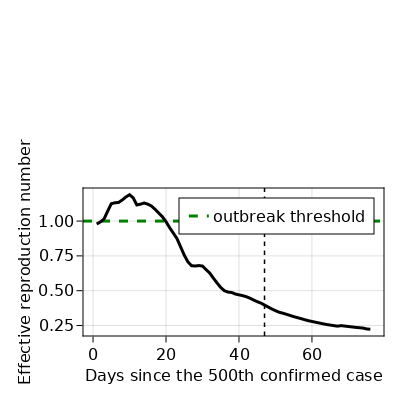
\includegraphics[width=\linewidth]{fb1/losangeles_ca/20211216180602.fbmobility1.losangeles_ca.R_effective.png}
        \end{subfigure}
        \begin{subfigure}[b]{0.4\linewidth}
            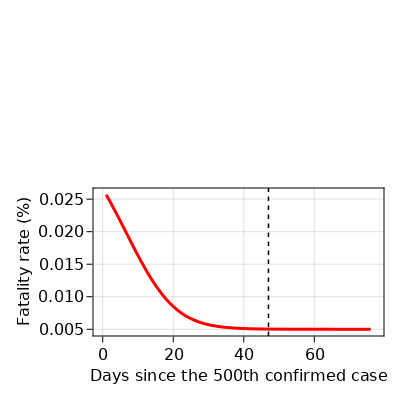
\includegraphics[width=\linewidth]{fb1/losangeles_ca/20211216180602.fbmobility1.losangeles_ca.fatality_rate.png}
        \end{subfigure}
        \subcaption{2nd. version}
    \end{subfigure}

    \begin{subfigure}[b]{\linewidth}
        \centering
        \begin{subfigure}[b]{0.4\linewidth}
            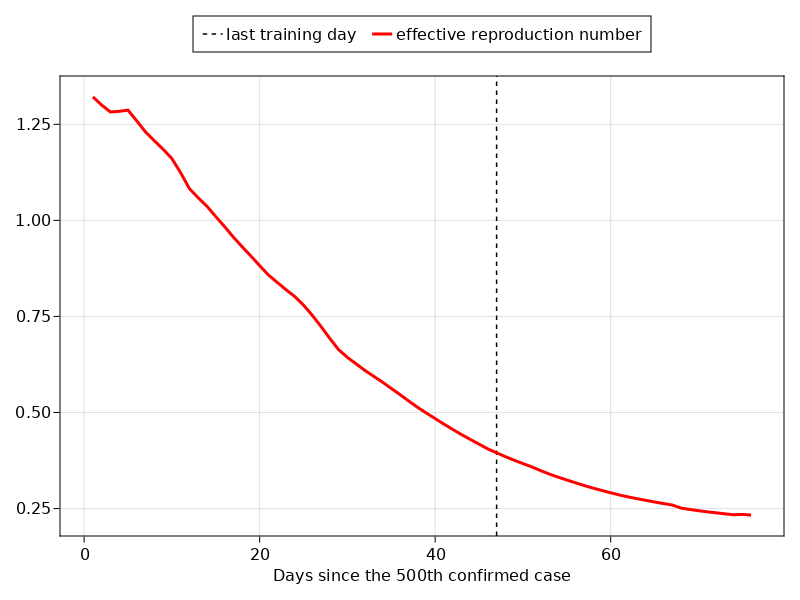
\includegraphics[width=\linewidth]{fb2/losangeles_ca/20211216142727.fbmobility2.losangeles_ca.R_effective.png}
        \end{subfigure}
        \begin{subfigure}[b]{0.4\linewidth}
            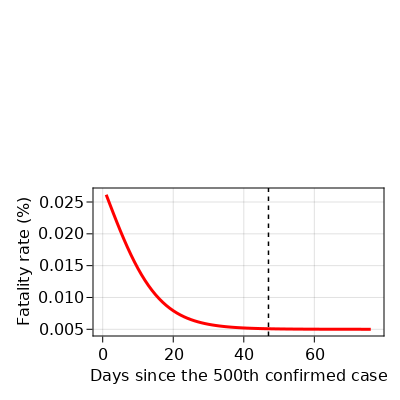
\includegraphics[width=\linewidth]{fb2/losangeles_ca/20211216142727.fbmobility2.losangeles_ca.fatality_rate.png}
        \end{subfigure}
        \subcaption{3rd. version}
    \end{subfigure}

    \caption{The effective reproduction number and the fatality rate for Los Angeles (California) learned by different versions of the model}
    \label{fig:R0-and-fatality-losangeles}
\end{figure}

\begin{figure}[!htb]
    \centering

    \begin{subfigure}[b]{\linewidth}
        \centering
        \begin{subfigure}[b]{0.4\linewidth}
            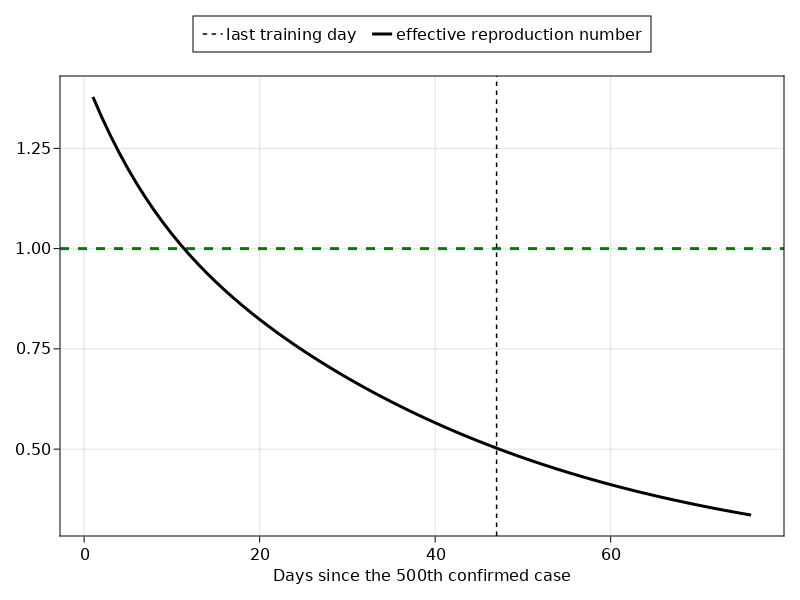
\includegraphics[width=\linewidth]{baseline/maricopa_az/20211216154445.baseline.maricopa_az.R_effective.png}
        \end{subfigure}
        \begin{subfigure}[b]{0.4\linewidth}
            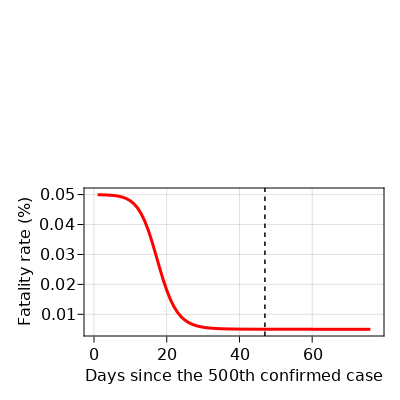
\includegraphics[width=\linewidth]{baseline/maricopa_az/20211216154445.baseline.maricopa_az.fatality_rate.png}
        \end{subfigure}
        \subcaption{Baseline model}
    \end{subfigure}

    \begin{subfigure}[b]{\linewidth}
        \centering
        \begin{subfigure}[b]{0.4\linewidth}
            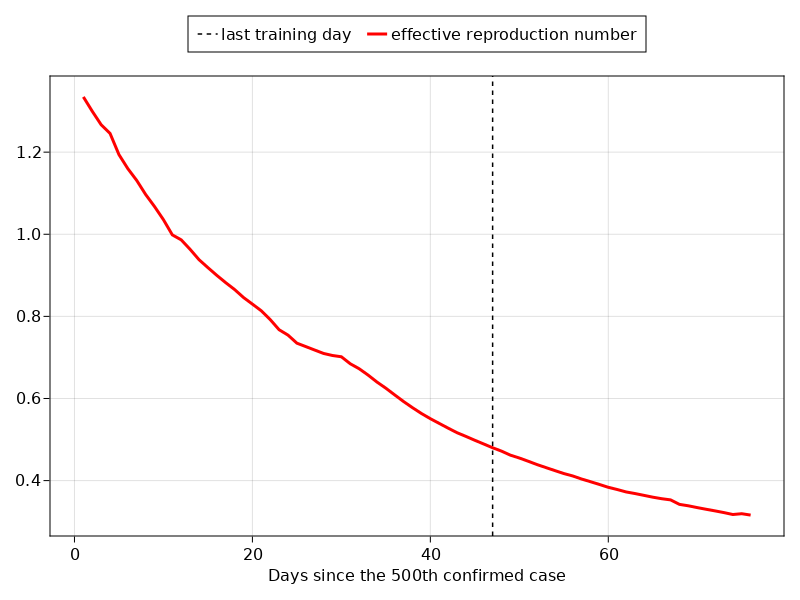
\includegraphics[width=\linewidth]{fb1/maricopa_az/20211216131821.fbmobility1.maricopa_az.R_effective.png}
        \end{subfigure}
        \begin{subfigure}[b]{0.4\linewidth}
            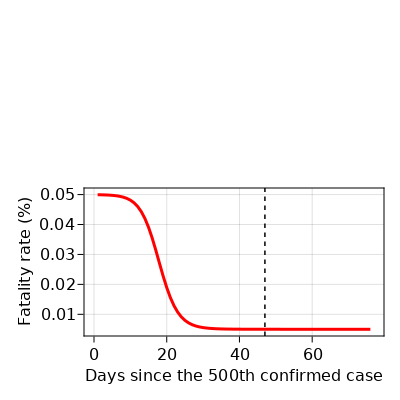
\includegraphics[width=\linewidth]{fb1/maricopa_az/20211216131821.fbmobility1.maricopa_az.fatality_rate.png}
        \end{subfigure}
        \subcaption{2nd. version}
    \end{subfigure}

    \begin{subfigure}[b]{\linewidth}
        \centering
        \begin{subfigure}[b]{0.4\linewidth}
            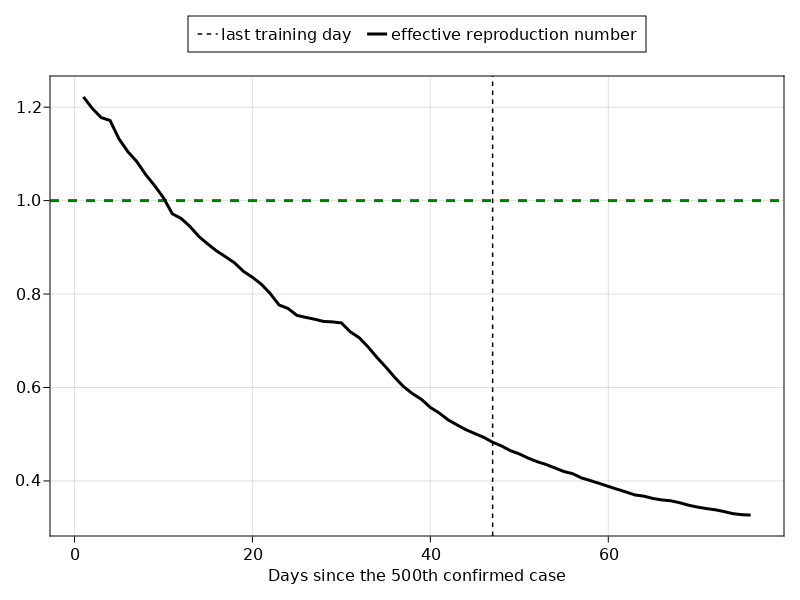
\includegraphics[width=\linewidth]{fb2/maricopa_az/20211216193717.fbmobility2.maricopa_az.R_effective.png}
        \end{subfigure}
        \begin{subfigure}[b]{0.4\linewidth}
            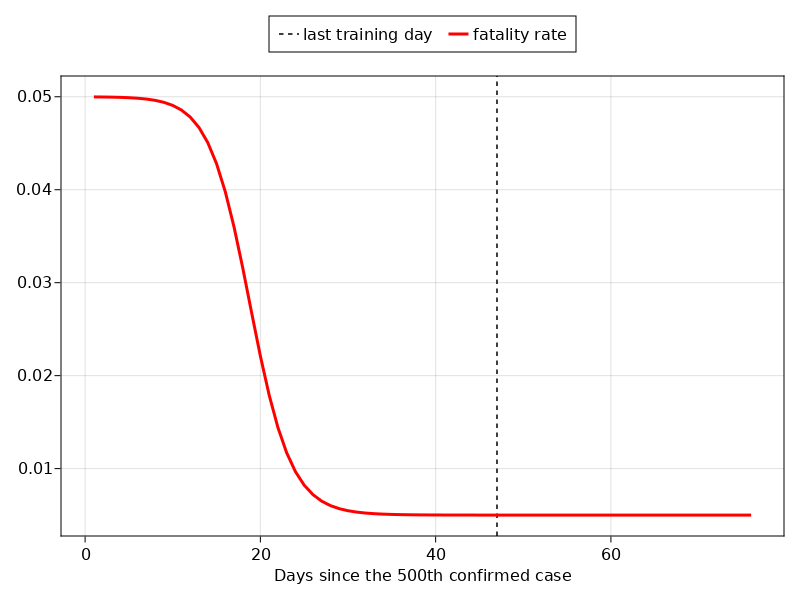
\includegraphics[width=\linewidth]{fb2/maricopa_az/20211216193717.fbmobility2.maricopa_az.fatality_rate.png}
        \end{subfigure}
        \subcaption{3rd. version}
    \end{subfigure}

    \caption{The effective reproduction number and the fatality rate for Maricopa (Arizona) learned by different versions of the model}
    \label{fig:R0-and-fatality-marico}
\end{figure}
